\documentclass[a4paper, 12pt, twoside]{article}
\usepackage[T2A,T1]{fontenc}
\usepackage[utf8]{inputenc}
\usepackage[english, russian]{babel}
\usepackage{graphicx}
\usepackage{ amssymb }
\usepackage[hcentering, bindingoffset = 10mm, right = 15 mm, left = 15 mm, top=20mm, bottom = 20 mm]{geometry}
\usepackage{multirow}
\usepackage{lipsum}
\usepackage{amsmath, amstext}
\usepackage{siunitx}
\usepackage{subcaption}
\usepackage{wrapfig}
\usepackage{adjustbox}
\usepackage{enumerate, indentfirst, float}
\usepackage{capt-of, svg}
\usepackage{ctable}
\usepackage{cmap} % Улучшенный поиск русских слов в полученном pdf-файле
\newcommand*{\hm}[1]{#1\nobreak\discretionary{} 
	{\hbox{$\mathsurround=0pt #1$}}{}}

\usepackage{pscyr} % Нормальные шрифты
\usepackage[normalem]{ulem} % для подчёркиваний uline
\ULdepth = 0.16em

\usepackage{fancyhdr} %Колонтикулы
\pagestyle{fancy}
\lhead{
\includegraphics[width = 10 mm]{logo.jpg} Лабораторная работа № 3.2.2}
\rhead{\textit{\today}}

\newenvironment{bottompar}{\par\vspace*{\fill}}{\clearpage}
 
\begin{document}
\begin{titlepage}

\newcommand{\HRule}{\rule{\linewidth}{0.7mm}} % Defines a new command for the horizontal lines, change thickness here

\center % Center everything on the page
 
%----------------------------------------------------------------------------------------
%	HEADING SECTIONS
%----------------------------------------------------------------------------------------

\textsc{\LARGE Московский Физико-Технический Институт}\\[1,5cm] % Name of your university/college
\textsc{\Large Кафедра общей физики}\\[0.5cm] % Major heading such as course name
\textsc{\large Лабораторная работа \textnumero  3.2.2}\\[0.5cm] % Minor heading such as course title

%----------------------------------------------------------------------------------------
%	TITLE SECTION
%----------------------------------------------------------------------------------------

\HRule
\\[0.4cm]
{ \huge \bfseries Резонанс напряжений.}
\\[0.2cm] % Title of your document
\HRule
\\[1.5cm]


 
%----------------------------------------------------------------------------------------
%	AUTHOR SECTION
%----------------------------------------------------------------------------------------

\begin{minipage}{0.4\textwidth}
	\begin{flushleft} \large
		\textbf{Автор:}\\
		Глеб Уваркин \\
		615 группа
	\end{flushleft}
\end{minipage}
~
\begin{minipage}{0.4\textwidth}
	\begin{flushright} \large
		\textbf {Преподаватель:} \\
		Андрей Александрович Заболотных % Supervisor's Name
	\end{flushright}
\end{minipage}

\begin{bottompar}
	\begin{center}
		
\includegraphics[width = 80 mm]{logo.jpg}
	\end{center}
	{\large \today}

\end{bottompar}
\vfill % Fill the rest of the page with whitespace

\end{titlepage}

{\Large \uline { \textbf  {Цель работы:}}}

\vspace{2mm}
Изучение последовательной цепи переменного тока, наблюдение резонанса напряжений.
\vspace{\baselineskip}

{\Large \uline { \textbf  {В работе используются:}}}

\vspace{2mm}

Регулировочный автотрансформатор, катушка индуктивности с выдвижным сердечником, магазин ёмкостей, реостат, резистор, амперметр, три вольтметра, ваттметр, осциллограф, универсальный мост.

\section{Теоретические сведения.}
\begin{figure}[H]
		\centering
		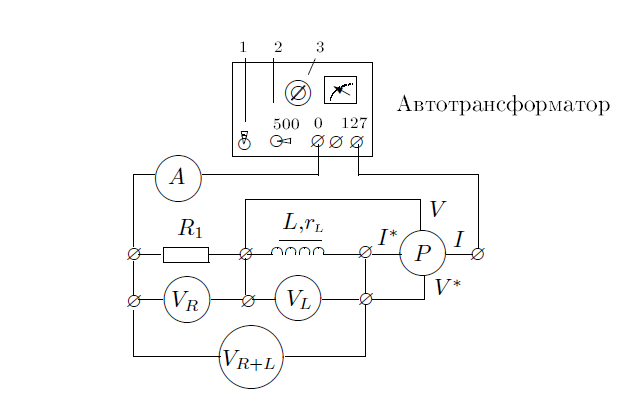
\includegraphics[width = 0.7\linewidth]{sch1}
		\caption{Схема установки для изучения закона Ома в цепи переменного тока.}
		\label{sch:1}
\end{figure}

Рассмотрим электрическую цепь, состоящую из резистора $R$ и катушки индуктивности $L$ с импедансом $Z_L = r_L+i\Omega L$, последовательно подключённых к внешнему источнику, ЭДС которого меняется по синусоидальному закону с частотой $\Omega$ (рис \ref{sch:1}).


Обозначим через $U_R$ напряжение на резисторе, через $U_L$ -- напряжение на катушке и через $U_{R+L}$ -- суммарное напряжение на катушке и на резисторе. Для этих напряжений справедливы комплексные соотношения:
\begin{equation}
\label{eq1}
\widehat{U}_R = \widehat{I}R,~\widehat{U}_L=\widehat{I}(r_L+i\omega L),~ \widehat{U}_{R+L} = \widehat{I}(R+r_L+i\Omega L)
\end{equation}

где $r_L$ -- активное сопротивление катушки, которое характеризует суммарные потери энергии в катушке, в том числе потери в её ферромагнитном сердечнике.

Переходя к модулям и фазам токов и напряжений, найдём из \eqref{eq1}:
\begin{equation}
\label{eq2}
U_R = I \cdot R,~~~~tg \psi_1 = 0
\end{equation}

\begin{equation}
\label{eq3}
U_L = I\cdot \sqrt{r_L^2+(\Omega L)^2},~~~~ tg \psi_2 = \dfrac{\Omega L}{r_L}
\end{equation}

\begin{equation}
\label{eq4}
U_{R+L} = I\sqrt{(R+r_L)^2+(\Omega L)^2},~~~~tg \psi_3 = \dfrac{\Omega L}{R+r_L}.
\end{equation}

В этих формулах $U$ и $I$ обозначают \textit{эффективные} значения напряжений и токов (показания приборов), как принято в электротехнике.

Измеряя с помощью трёх вольтметров значения $U_R,~U_L$ и $U_{R+L}$ и зная сопротивление резистора $R$, нетрудно вычислить, пользуясь формулами \eqref{eq2}, \eqref{eq3} и \eqref{eq4}, силу тока в цепи, активное сопротивление катушки $r_L$, её индуктивность L, мощность $P_L$, выделяемую на катушке, и сдвиг фаз между током и напряжением на катушке.

Рассчитаем мощность переменного тока, выделяемую в катушке. Мгновенное значение мощности равно
$$P = U(t)\cdot I(t).$$

Средняя мощность за период $T$ определяется формулой 
$$\overline{P} = \dfrac{1}{T}\int\limits_0^T U(t) \cdot I(t) dt$$.

Полагая $I(t) = I\sqrt{2}\cos \Omega t,~U(t) = U\sqrt{2}\cos(\Omega t+\psi)$, получим после интегрирования:

\begin{equation}
\label{eq5}
P_L = U_L\cdot I \cos \psi = I^2\cdot r_L.
\end{equation}

Средняя мощность, выделяющаяся в катушке самоиндукции, определяется, таким образом, действительной частью её импеданса.

Активное сопротивление катушки $r_L$ можно определить, если включить её в последовательный колебательный контур с известными параметрами -- сопротивлением $R$ и ёмкостью $C$ (рис.\ref{sch:2}). В контуре, настроенном в резонанс на частоту $\Omega$ внешнего источника (собственная частоту контура и внешняя совпадают: $\omega_0=\Omega$), реактивные сопротивления индуктивности и ёмкости одинаковы:
\begin{equation}
\label{eq:6}
\omega_0 L = \dfrac{1}{\omega_0 C}.
\end{equation}

Определив каким-либо экспериментальным способом добротность этого контура, можно рассчитать полное сопротивление контура $R_{\sum}$ в резонансе, поскольку 
\begin{equation}
\label{eq:7}
Q = \dfrac{\omega_0 L}{R_{\sum}} = \dfrac{1}{\omega_0 C R_{\sum}}.
\end{equation}

Резонансное сопротивление контура $R_{\sum}$ включает в себя известное сопротивление резистора $R$ и активное сопротивление катушки $r_L$:
\begin{equation}
\label{eq:8}
R_{\sum} = R + r_L.
\end{equation}


\section{Экспериментальная установка.}

Схема установки для исследования закона Ома в цепи переменного тока представлена на рис. \ref{sch:1}. Цепь, состоящая из резистора $R_1 \simeq 100~\text{Ом}$ и катушки $L$ с выдвижным сердечником, подключена к автотрансформатору, выходное напряжение которого можно менять от $0$ до $127$ В. Напряжение на каждом из элементов и суммарное напряжение цепи измеряются тремя вольтметрами: $V_R,~V_L,$ и $V_{R+L}$. Амперметр $A$ измеряет ток в цепи, а ваттметр $P$ -- мощность, выделяющуюся на катушке.

\begin{figure}[H]
	\centering
	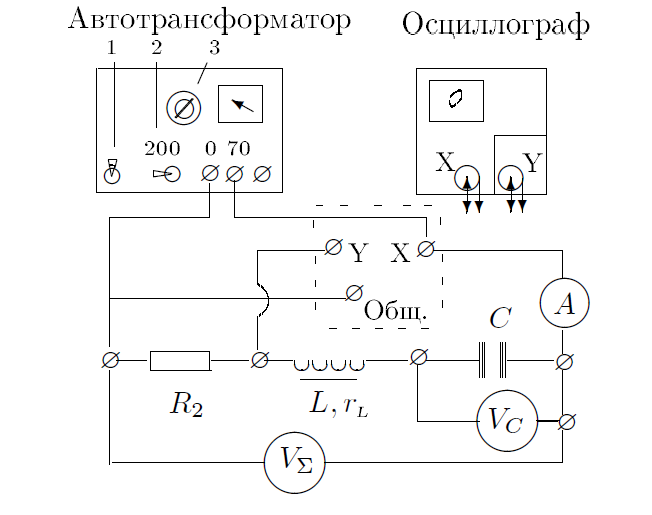
\includegraphics[width = 0.7\linewidth]{sch2}
	\caption{Схема установки для наблюдения резонанса напряжений.}
	\label{sch:2}
\end{figure}

Схема установки для изучения резонанса напряжений изображена на рис.\ref{sch:2}. Последовательно соединены резистор $R_2\simeq 5~\text{Ом}$, катушка $L$ и магазин ёмкостей $C$. Амперметр $A$ измеряет ток в цепи, вольтметр $V_C$ -- напряжение на ёмкости, вольтметр $V_{\sum}$ -- суммарное напряжение на контуре. Резонанс можно зафиксировать с помощью осциллографа, если подать на вход $X$ напряжение с контура, а на вход $Y$ -- напряжение с резистора $R_2$, пропорциональное току в цепи. В общем случае на экране виден эллипс. При резонансе эллипс вырождается в прямую линию.

Резонансные напряжения на контуре $U_{\sum,\text{рез}}$ и на ёмкости $U_{C,\text{рез}}$ равны соответственно

\begin{equation}
\label{eq:9}
U_{\sum,\text{рез}} = I_{\text{рез}}R_{\sum},~~~~U_{C,\text{рез}} = \dfrac{I_\text{рез}}{\Omega C}
\end{equation}

Сравнивая \eqref{eq:7} и \eqref{eq:9}, получим 

\begin{equation}
\label{eq:10}
Q = \dfrac{U_{C,\text{рез}}}{U_{\sum,\text{рез}}}
\end{equation}

Формула \eqref{eq:10} показывает, что добротность контура может быть найдена по измеренным значениям напряжений на контуре и на конденсаторе при резонансе. Зная добротность контура и ёмкость $C$, можно рассчитать $R_{\sum}$ по формуле \eqref{eq:7}, а затем определить $r_L$.

\newpage
\section{Обработка результатов.}
\subsection{Закон Ома в цепи переменного тока.}

Перемещая сердечник шагами по $2$ м, снимем зависимость тока $I$, напряжений $U_R,~U_L,~U_{R+L}$ и мощности $P_L$ от координаты сердечника $x$. По результатам измерений $P_L$ и $I$ вычислим значение $r_L$ по формуле \eqref{eq5}, а также, зная частоту сети $\nu_0 = 50~\text{Гц}$, определим $L$ с помощью \eqref{eq3}:

\begin{table}[H]
	\centering
	\caption{Определение $r_L$ и $L$.}
	\label{t1}
	\begin{tabular}{c|ccccccccccc} \toprule
		$x,~\text{мм}$           & 3  & 5 & 7  & 9  & 10  & 11 & 13 & 15   & 17   & 19 & 21 \\
		$\sigma_{x},~\text{мм}$ & \multicolumn{11}{c}{0.5}                                                        \\ \midrule
		$I \cdot 10^{-1},~A$           & 5.25  & 7.25 & 8.50  & 9.00  & 9.25  & 9.50 & 9.75 & 10.00   & 10.13   & 10.25 & 10.50 \\
		$\sigma_{I}\cdot 10^{-1},~A$ & \multicolumn{11}{c}{0.25}                                                        \\ \midrule
		$P_L,~\text{Вт}$                & 15.75 & 13   & 11.25 & 10.50 & 10.25 & 9.75 & 9.00 & 8.75 & 8.25 & 8     & 7.75  \\
		$\sigma_{P_L},~\text{Вт}$      & \multicolumn{11}{c}{0.25}   \\ \midrule
		$r_L,~\text{Ом}$                & 57.1 & 24.7   & 15.6 & 12.9 & 11.9 & 10.8 & 9.47 & 8.8 & 8.0 & 7.6     & 7.0 \\ 
		$\sigma_{r_L},~\text{Ом}$      &3.9 &1.3&0.7&0.6&0.5&0.5&0.4&0.4&0.4&0.4&0.3 \\ \midrule
		$U_L,~\text{В}$                & 102 & 87   & 71 & 69 & 63 & 61 & 58 & 54 & 51 & 49 & 46 \\ 
		$\sigma_{U_L},~\text{В}$      & \multicolumn{11}{c}{1} \\ \midrule
		$L\cdot 10^{-2},~\text{Гн}$                & 59.1 &37.4    & 26.1 & 24.1 & 21.4 & 20.2 & 18.7 & 16.9 & 15.8 & 15.0     & 13.8 \\ 
		$\sigma_{L}\cdot 10^{-2},~\text{Гн}$      &5.0 &2.4  &1.5  &1.3  &1.2  &1.1  &1.0  &0.9  &0.9  &0.8  &0.8 \\ \bottomrule                                                    
	\end{tabular}
\end{table}

Построим графики зависимостей $L$ и $r_L$ от положения сердечника и определим по ним значения $L$ и $r_L$, соответствующее среднему (резонансному) положению сердечника.

\begin{figure}[H]
	\centering
	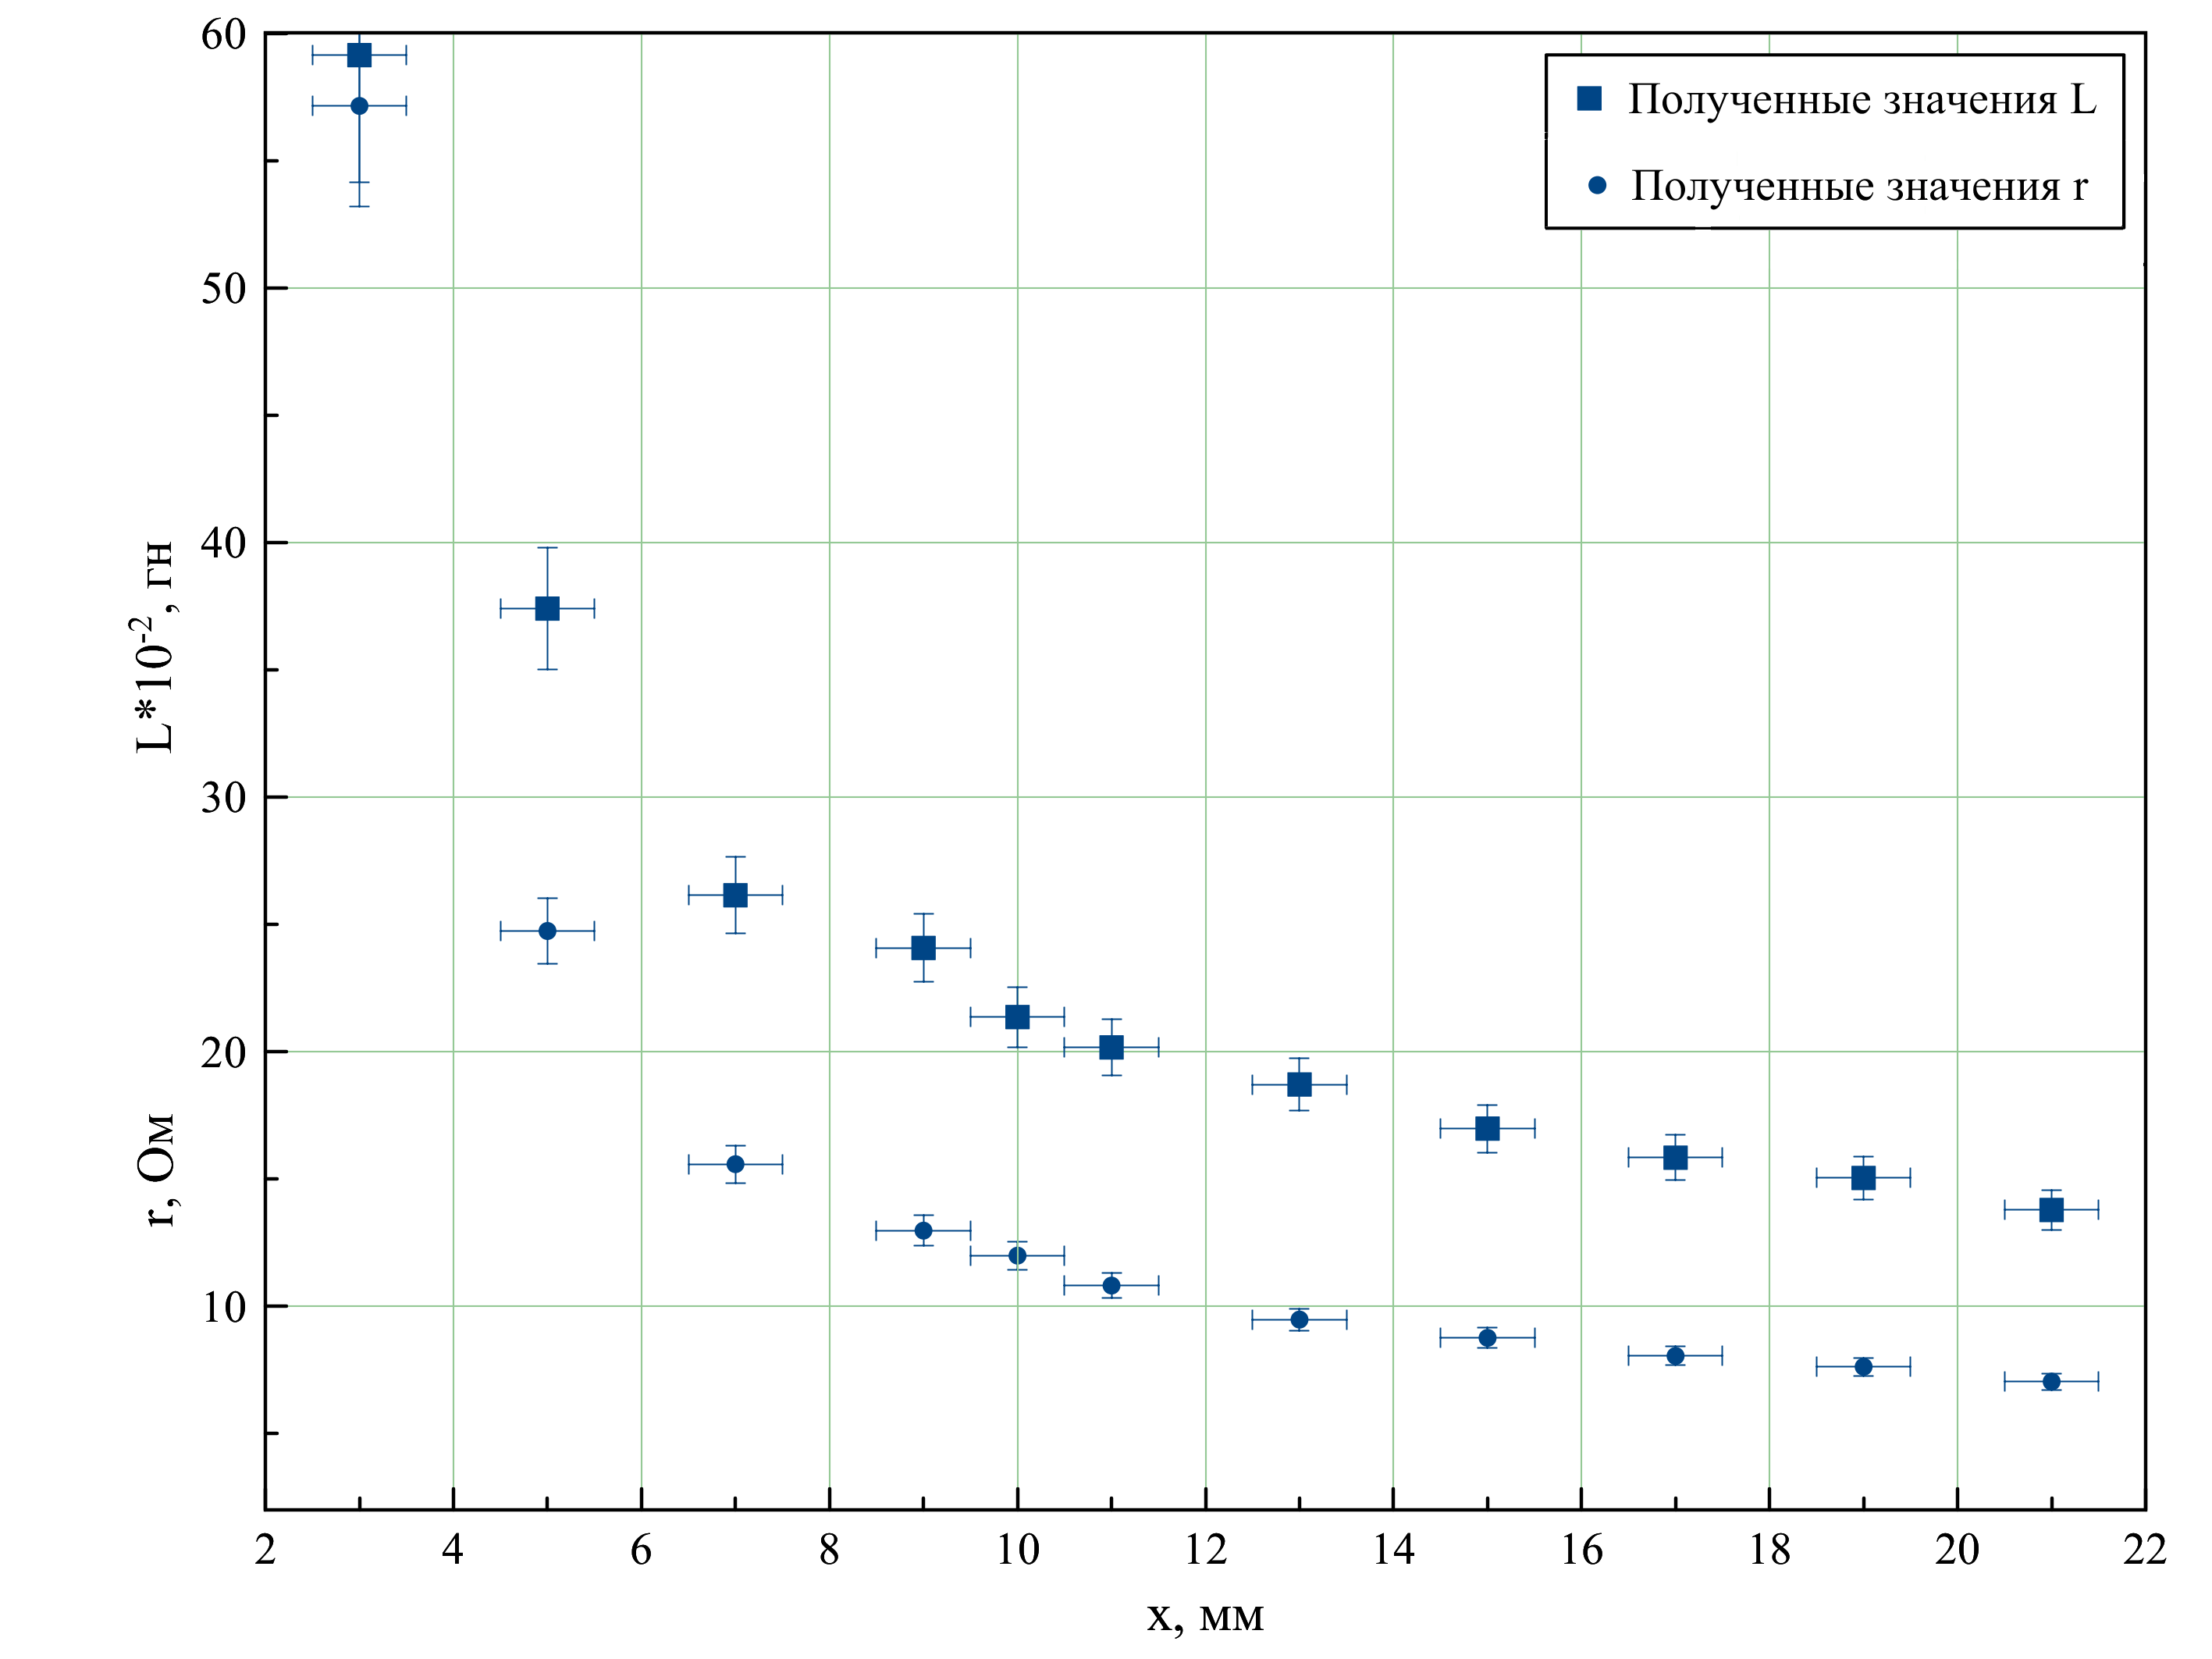
\includegraphics[width = 0.8\linewidth]{itog}
	\caption{Зависимость $L$ и $r_L$ от положения сердечника.}
\end{figure}

$$L \simeq (214\pm 12)~\text{мГн}~(\varepsilon \simeq 5.6 \%),~~r_L \simeq (11.9 \pm 0.5)~\text{Ом}~(\varepsilon \simeq 4.2 \%)$$


Для среднего положения сердечника построим векторную диаграмму напряжений. Отложим на диаграмме активную ($U_{L,~\text{акт}}$) и реактивную ($U_{L,~\text{реакт}}$) составляющие напряжения на катушке и рассчитаем по ним значения $L$ и $r_L$.

\begin{minipage}{0.3\linewidth}
	\begin{table}[H]
		\centering
		\caption{Показания вольтметров и амперметра при среднем положении сердечника.}
		\begin{tabular}{c|c|c|c}\toprule
			$U_R,~\text{В}$ & $U_{R+L},~\text{В}$ & $U_L,~\text{В}$ & $I,~\text{А}$ \\ \midrule
			83              & 114                 & 63  & 0.925 \\ \bottomrule            
		\end{tabular}
	\end{table}
\end{minipage}
~
\begin{minipage}{0.69\linewidth}
\begin{figure}[H]
	\centering
	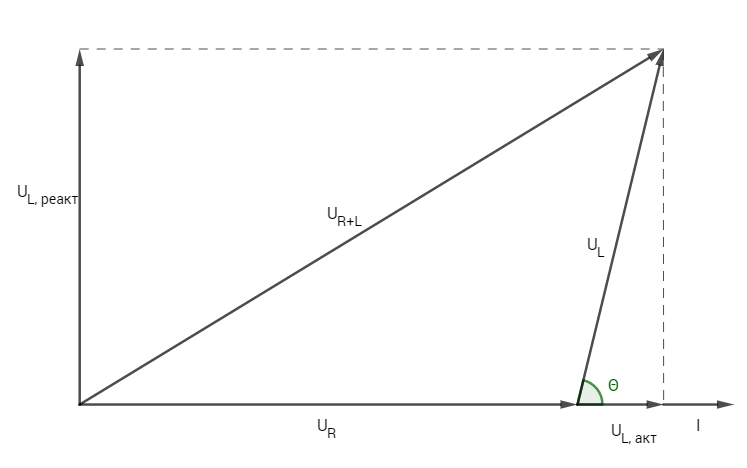
\includegraphics[width = 0.8\linewidth]{vdiagr}
	\caption{Векторная диаграмма.}
\end{figure}
\end{minipage}

~

По теореме косинусов получаем:
$$\cos \theta = -\dfrac{U_R^2+U_L^2-U_{R+L}^2}{2U_R U_L} \simeq 0.204 \pm 0.004$$

Отсюда имеем:
$$U_{L,~\text{акт}} = U_L  \cos \theta \simeq (12.85 \pm 0.32)~\text{В}$$
$$U_{L,~\text{реакт}} = U_L \sqrt{1-\cos^2 \theta} \simeq (61.68 \pm 1.56)~\text{В}.$$
$$U_{L,~\text{акт}} = I\cdot r_L ~ \Rightarrow ~ r_L = \dfrac{U_{L,~\text{акт}}}{I}\simeq (13.89 \pm 0.51)~\text{Ом}~(\varepsilon \simeq 3.7\%)$$
$$U_{L,~\text{реакт}} = I\Omega L ~ \Rightarrow ~ L = \dfrac{U_{L,~\text{реакт}}}{I\Omega} \simeq (212.4 \pm 7.9)~\text{мГн}~(\varepsilon \simeq 3.7 \%).$$

Рассчитаем $\cos \theta$ по формуле \eqref{eq5}:
$$\cos \theta = \dfrac{P_L}{U_L\cdot I} \simeq 0.176 \pm 0.007.$$

Значения $\cos \theta$, полученное с помощью векторной диаграммы и рассчитанное по формуле \eqref{eq5}, очень близки.

С помощью векторной диаграммы по теореме косинусов рассчитаем мощность $P_L$, выделяемую на катушке, через напряжения $U_R,~U_L,~U_{R+L}$ и сопротивление $R_1 = 98~\text{Ом}$ (метол трёх вольтметров).

$$P_L = U_L I \cos\theta = U_L \dfrac{U_R}{R_1}\cos\theta \simeq (10.88 \pm 0.30)~\text{Вт}.$$

\subsection{Резонанс напряжений.}

Рассчитаем активное сопротивление катушки $r_L$ через ток и напряжение на контуре (формулы \eqref{eq:8} и \eqref{eq:9}).
$$ r_L = \dfrac{U_{\sum,~ \text{рез}}}{I_{\text{рез}}} - R_2 = \dfrac{31}{3.05} - 5.6 = (4.56 \pm 0.10)~ \text{Ом}~(\varepsilon \simeq 2.2\%) $$

Рассчитаем $L$ и $r_L$ через добротность (формулы \eqref{eq:10}, \eqref{eq:6}, \eqref{eq:7}, \eqref{eq:8}):
$$Q = \dfrac{U_{C,~\text{рез}}}{U_{\sum,~\text{рез}}} = \dfrac{230}{31} \simeq 7.42 \pm 0.14$$

$$r_L = \dfrac{1}{Q\omega_0 C} - R_2 = \dfrac{1}{7.42 \cdot 2\pi \cdot 50\cdot 42.6\cdot 10^{-6}} - 5.6 \simeq (4.48 \pm 0.24)~\text{Ом}~(\varepsilon \simeq 5.4\%)$$

$$L = \dfrac{(r_L+R_2)Q}{\omega_0} = \dfrac{10.07\cdot 7.42}{2\pi \cdot 50} \simeq (238 \pm 14)~\text{мГн}~(\varepsilon \simeq 5.9\%).$$

Занесём результаты в таблицу:

\begin{table}[H]
	\centering
	\caption{Полученные значения.}
	\begin{tabular}{c|c|c|c|c|c} \toprule
		& Мост E7- & График & Вект.диагр & $f(I_{\text{рез}},U_{\sum,~\text{рез}})$ & f(Q) \\ \midrule
		$r_L,~\text{Ом}$ & $4.86$         & $11.9\pm 0.5$       & $13.9 \pm 0.5$           &$4.56 \pm 0.10$                                    &$4.48 \pm 0.24$      \\
		$L,~\text{мГн}$  & $202$         &  $214 \pm 12$      &   $212 \pm 8$         &     -                                     &$238 \pm 14$  \\ \bottomrule   
	\end{tabular}
\end{table}

\section{Вывод.}

Значения индуктивности катушки, полученные разными способами, практически совпадают, а значения активного сопротивления катушки, измеренные с помощью разных цепей (в рамках одной цепи значения близки), различаются. Это может быть связано с тем, что в цепи, изображенной на рис.(\ref{sch:1}) сила тока была около $1$ A, а в цепи, изображенной на рис.(\ref{sch:2}) -- $3$ A, а, как известно, активное сопротивление катушки зависит от частоты и амплитуды тока.





\end{document}

